

\tikzset{every picture/.style={line width=0.75pt}} %set default line width to 0.75pt

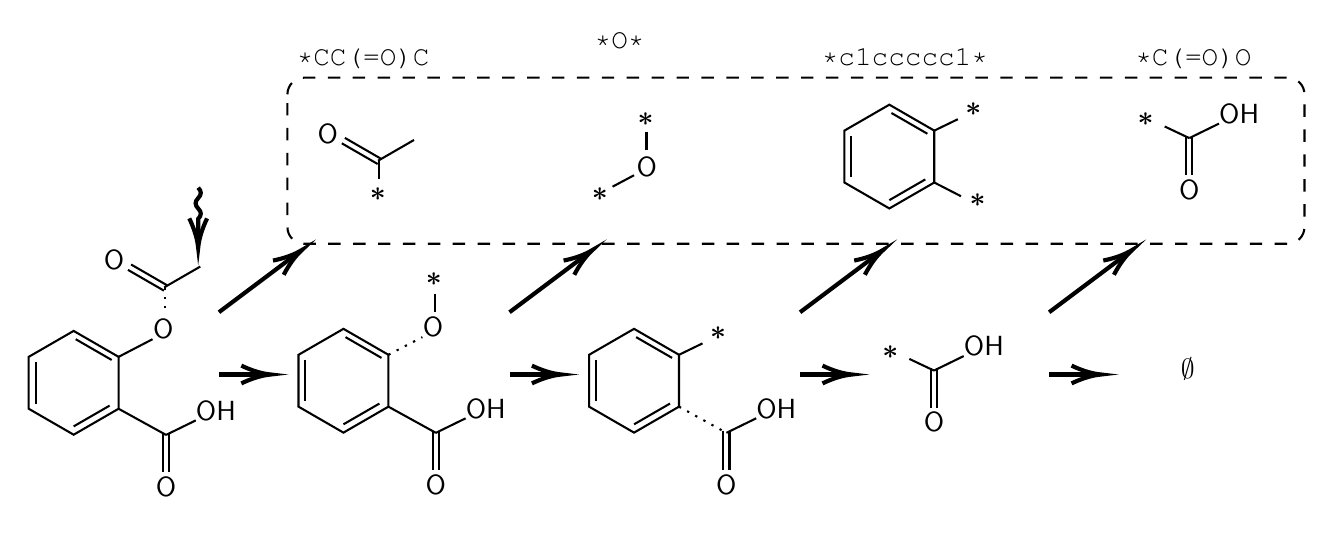
\begin{tikzpicture}[x=0.75pt,y=0.75pt,yscale=-1,xscale=1]
%uncomment if require: \path (0,261); %set diagram left start at 0, and has height of 261

%Shape: Regular Polygon [id:dp5441528921455343]
\draw   (40,219) -- (18.35,206.5) -- (18.35,181.5) -- (40,169) -- (61.65,181.5) -- (61.65,206.5) -- cycle ;
%Straight Lines [id:da8353669023127415]
\draw [color={rgb, 255:red, 0; green, 0; blue, 0 }  ,draw opacity=1 ] [dash pattern={on 0.84pt off 2.51pt}]  (84,148) -- (84,161) ;
%Straight Lines [id:da7264741738633573]
\draw    (61.65,206.5) -- (84.52,219.11) ;
%Straight Lines [id:da9419897329918221]
\draw    (83,218) -- (83,237) ;
%Straight Lines [id:da08030707542558835]
\draw    (86,218) -- (86,237) ;
%Straight Lines [id:da5530700734644509]
\draw    (66.18,139.6) -- (83.5,149.6) ;
%Straight Lines [id:da790594687957088]
\draw    (67.68,137) -- (85,147) ;
%Straight Lines [id:da9254167439072243]
\draw    (101,138) -- (83.68,148) ;
%Straight Lines [id:da8637172136187801]
\draw    (98.84,212.11) -- (84.52,219.11) ;
%Shape: Boxed Line [id:dp15467998486140555]
\draw    (58.32,183) -- (41,173) ;
%Shape: Boxed Line [id:dp7874277710723612]
\draw    (21.66,184) -- (21.66,204) ;
%Shape: Boxed Line [id:dp7393760826446616]
\draw    (57.32,205) -- (40,215) ;
%Straight Lines [id:da6253733493164098]
\draw    (61.65,181.5) -- (78,173) ;
%Straight Lines [id:da14339200969487864]
\draw    (187,87) -- (187,96) ;
%Straight Lines [id:da44923721765501834]
\draw    (169.18,78.6) -- (186.5,88.6) ;
%Straight Lines [id:da7396190068173174]
\draw    (170.68,76) -- (188,86) ;
%Straight Lines [id:da2642417615054462]
\draw    (204,77) -- (186.68,87) ;
%Shape: Regular Polygon [id:dp7544269598266076]
\draw   (170,218) -- (148.35,205.5) -- (148.35,180.5) -- (170,168) -- (191.65,180.5) -- (191.65,205.5) -- cycle ;
%Straight Lines [id:da39600377387545027]
\draw    (214,151) -- (214,160) ;
%Straight Lines [id:da34587108939367583]
\draw    (191.65,205.5) -- (214.52,218.11) ;
%Straight Lines [id:da16212666985437285]
\draw    (213,217) -- (213,236) ;
%Straight Lines [id:da27990188760620915]
\draw    (216,217) -- (216,236) ;
%Straight Lines [id:da12782422389072567]
\draw    (228.84,211.11) -- (214.52,218.11) ;
%Shape: Boxed Line [id:dp12710407729792883]
\draw    (188.32,182) -- (171,172) ;
%Shape: Boxed Line [id:dp06901241168496686]
\draw    (151.66,183) -- (151.66,203) ;
%Shape: Boxed Line [id:dp24332035305461464]
\draw    (187.32,204) -- (170,214) ;
%Straight Lines [id:da4254972054869146]
\draw [color={rgb, 255:red, 0; green, 0; blue, 0 }  ,draw opacity=1 ] [dash pattern={on 0.84pt off 2.51pt}]  (191.65,180.5) -- (208,172) ;
%Straight Lines [id:da35759409213918647]
\draw    (316,73) -- (316,82) ;
%Straight Lines [id:da5439851805644256]
\draw    (299.65,99.5) -- (310,94) ;
%Shape: Regular Polygon [id:dp5780688789268227]
\draw   (310,218) -- (288.35,205.5) -- (288.35,180.5) -- (310,168) -- (331.65,180.5) -- (331.65,205.5) -- cycle ;
%Straight Lines [id:da7189531753769425]
\draw [color={rgb, 255:red, 0; green, 0; blue, 0 }  ,draw opacity=1 ] [dash pattern={on 0.84pt off 2.51pt}]  (331.65,205.5) -- (354.52,218.11) ;
%Straight Lines [id:da015729760849670926]
\draw    (353,217) -- (353,236) ;
%Straight Lines [id:da508744745614957]
\draw    (356,217) -- (356,236) ;
%Straight Lines [id:da7333901214969005]
\draw    (368.84,211.11) -- (354.52,218.11) ;
%Shape: Boxed Line [id:dp7821116031259598]
\draw    (328.32,182) -- (311,172) ;
%Shape: Boxed Line [id:dp2991980751528647]
\draw    (291.66,183) -- (291.66,203) ;
%Shape: Boxed Line [id:dp23007592478514582]
\draw    (327.32,204) -- (310,214) ;
%Straight Lines [id:da7839141780584493]
\draw    (331.65,180.5) -- (343,175) ;
%Shape: Regular Polygon [id:dp06504553344048047]
\draw   (433,110) -- (411.35,97.5) -- (411.35,72.5) -- (433,60) -- (454.65,72.5) -- (454.65,97.5) -- cycle ;
%Straight Lines [id:da5415663535410995]
\draw    (454.65,97.5) -- (467.52,104.11) ;
%Shape: Boxed Line [id:dp6678344578633082]
\draw    (451.32,74) -- (434,64) ;
%Shape: Boxed Line [id:dp8151982232927417]
\draw    (414.66,75) -- (414.66,95) ;
%Shape: Boxed Line [id:dp7238017036812237]
\draw    (450.32,96) -- (433,106) ;
%Straight Lines [id:da9324796829842863]
\draw    (454.65,72.5) -- (466,67) ;
%Straight Lines [id:da5149286578798244]
\draw    (442.65,182.5) -- (454.52,188.11) ;
%Straight Lines [id:da19919766764775115]
\draw    (453,187) -- (453,206) ;
%Straight Lines [id:da3191045376521391]
\draw    (456,187) -- (456,206) ;
%Straight Lines [id:da7608894861911997]
\draw    (468.84,181.11) -- (454.52,188.11) ;
%Straight Lines [id:da2833824315266147]
\draw    (565.65,70.5) -- (577.52,76.11) ;
%Straight Lines [id:da021587565605220016]
\draw    (576,75) -- (576,94) ;
%Straight Lines [id:da764675922133226]
\draw    (579,75) -- (579,94) ;
%Straight Lines [id:da4168629259527994]
\draw    (591.84,69.11) -- (577.52,76.11) ;
%Shape: Rectangle [id:dp8768800468171065]
\draw  [dash pattern={on 4.5pt off 4.5pt}] (143,55) .. controls (143,50.58) and (146.58,47) .. (151,47) -- (625,47) .. controls (629.42,47) and (633,50.58) .. (633,55) -- (633,119) .. controls (633,123.42) and (629.42,127) .. (625,127) -- (151,127) .. controls (146.58,127) and (143,123.42) .. (143,119) -- cycle ;
%Straight Lines [id:da2386684232536831]
\draw [line width=1.5]    (110,160) -- (147.6,131.8) ;
\draw [shift={(150,130)}, rotate = 503.13] [color={rgb, 255:red, 0; green, 0; blue, 0 }  ][line width=1.5]    (14.21,-4.28) .. controls (9.04,-1.82) and (4.3,-0.39) .. (0,0) .. controls (4.3,0.39) and (9.04,1.82) .. (14.21,4.28)   ;
%Straight Lines [id:da654107192310643]
\draw [line width=1.5]    (110,190) -- (132,190) ;
\draw [shift={(135,190)}, rotate = 180] [color={rgb, 255:red, 0; green, 0; blue, 0 }  ][line width=1.5]    (14.21,-4.28) .. controls (9.04,-1.82) and (4.3,-0.39) .. (0,0) .. controls (4.3,0.39) and (9.04,1.82) .. (14.21,4.28)   ;
%Straight Lines [id:da7007314823593822]
\draw [line width=1.5]    (250,160) -- (287.6,131.8) ;
\draw [shift={(290,130)}, rotate = 503.13] [color={rgb, 255:red, 0; green, 0; blue, 0 }  ][line width=1.5]    (14.21,-4.28) .. controls (9.04,-1.82) and (4.3,-0.39) .. (0,0) .. controls (4.3,0.39) and (9.04,1.82) .. (14.21,4.28)   ;
%Straight Lines [id:da9466136946677108]
\draw [line width=1.5]    (250,190) -- (272,190) ;
\draw [shift={(275,190)}, rotate = 180] [color={rgb, 255:red, 0; green, 0; blue, 0 }  ][line width=1.5]    (14.21,-4.28) .. controls (9.04,-1.82) and (4.3,-0.39) .. (0,0) .. controls (4.3,0.39) and (9.04,1.82) .. (14.21,4.28)   ;
%Straight Lines [id:da30124943836314677]
\draw [line width=1.5]    (390,160) -- (427.6,131.8) ;
\draw [shift={(430,130)}, rotate = 503.13] [color={rgb, 255:red, 0; green, 0; blue, 0 }  ][line width=1.5]    (14.21,-4.28) .. controls (9.04,-1.82) and (4.3,-0.39) .. (0,0) .. controls (4.3,0.39) and (9.04,1.82) .. (14.21,4.28)   ;
%Straight Lines [id:da4416094050725605]
\draw [line width=1.5]    (390,190) -- (412,190) ;
\draw [shift={(415,190)}, rotate = 180] [color={rgb, 255:red, 0; green, 0; blue, 0 }  ][line width=1.5]    (14.21,-4.28) .. controls (9.04,-1.82) and (4.3,-0.39) .. (0,0) .. controls (4.3,0.39) and (9.04,1.82) .. (14.21,4.28)   ;
%Straight Lines [id:da7724041476627761]
\draw [line width=1.5]    (510,160) -- (547.6,131.8) ;
\draw [shift={(550,130)}, rotate = 503.13] [color={rgb, 255:red, 0; green, 0; blue, 0 }  ][line width=1.5]    (14.21,-4.28) .. controls (9.04,-1.82) and (4.3,-0.39) .. (0,0) .. controls (4.3,0.39) and (9.04,1.82) .. (14.21,4.28)   ;
%Straight Lines [id:da10439710720480422]
\draw [line width=1.5]    (510,190) -- (532,190) ;
\draw [shift={(535,190)}, rotate = 180] [color={rgb, 255:red, 0; green, 0; blue, 0 }  ][line width=1.5]    (14.21,-4.28) .. controls (9.04,-1.82) and (4.3,-0.39) .. (0,0) .. controls (4.3,0.39) and (9.04,1.82) .. (14.21,4.28)   ;
%Straight Lines [id:da6206515346709651]
\draw [line width=1.5]    (100,100) .. controls (101.67,101.67) and (101.67,103.33) .. (100,105) .. controls (98.33,106.67) and (98.33,108.33) .. (100,110) .. controls (101.67,111.67) and (101.67,113.33) .. (100,115) -- (100,118) -- (100,126) ;
\draw [shift={(100,129)}, rotate = 270] [color={rgb, 255:red, 0; green, 0; blue, 0 }  ][line width=1.5]    (14.21,-4.28) .. controls (9.04,-1.82) and (4.3,-0.39) .. (0,0) .. controls (4.3,0.39) and (9.04,1.82) .. (14.21,4.28)   ;

% Text Node
\draw (59.5,135) node   [align=left] {\begin{minipage}[lt]{8.67pt}\setlength\topsep{0pt}
\begin{center}
$\displaystyle \mathsf{O}$
\end{center}

\end{minipage}};
% Text Node
\draw  [draw opacity=0]  (74.7,162) -- (91.7,162) -- (91.7,174) -- (74.7,174) -- cycle  ;
\draw (83.2,168) node   [align=left] {\begin{minipage}[lt]{8.67pt}\setlength\topsep{0pt}
\begin{center}
$\displaystyle \mathsf{O}$
\end{center}

\end{minipage}};
% Text Node
\draw  [draw opacity=0][fill={rgb, 255:red, 255; green, 255; blue, 255 }  ,fill opacity=1 ]  (76,238) -- (93,238) -- (93,250) -- (76,250) -- cycle  ;
\draw (84.5,244) node   [align=left] {\begin{minipage}[lt]{8.67pt}\setlength\topsep{0pt}
\begin{center}
$\displaystyle \mathsf{O}$
\end{center}

\end{minipage}};
% Text Node
\draw  [draw opacity=0][fill={rgb, 255:red, 255; green, 255; blue, 255 }  ,fill opacity=1 ]  (96.2,198) -- (113.2,198) -- (113.2,210) -- (96.2,210) -- cycle  ;
\draw (104.7,204) node   [align=left] {\begin{minipage}[lt]{8.67pt}\setlength\topsep{0pt}
\begin{center}
$\displaystyle \mathsf{OH}$
\end{center}

\end{minipage}};
% Text Node
\draw (162.5,74) node   [align=left] {\begin{minipage}[lt]{8.67pt}\setlength\topsep{0pt}
\begin{center}
$\displaystyle \mathsf{O}$
\end{center}

\end{minipage}};
% Text Node
\draw (186.5,105) node   [align=left] {\begin{minipage}[lt]{8.67pt}\setlength\topsep{0pt}
\begin{center}
\textbf{*}
\end{center}

\end{minipage}};
% Text Node
\draw  [draw opacity=0]  (204.7,161) -- (221.7,161) -- (221.7,173) -- (204.7,173) -- cycle  ;
\draw (213.2,167) node   [align=left] {\begin{minipage}[lt]{8.67pt}\setlength\topsep{0pt}
\begin{center}
$\displaystyle \mathsf{O}$
\end{center}

\end{minipage}};
% Text Node
\draw  [draw opacity=0][fill={rgb, 255:red, 255; green, 255; blue, 255 }  ,fill opacity=1 ]  (206,237) -- (223,237) -- (223,249) -- (206,249) -- cycle  ;
\draw (214.5,243) node   [align=left] {\begin{minipage}[lt]{8.67pt}\setlength\topsep{0pt}
\begin{center}
$\displaystyle \mathsf{O}$
\end{center}

\end{minipage}};
% Text Node
\draw  [draw opacity=0][fill={rgb, 255:red, 255; green, 255; blue, 255 }  ,fill opacity=1 ]  (226.2,197) -- (243.2,197) -- (243.2,209) -- (226.2,209) -- cycle  ;
\draw (234.7,203) node   [align=left] {\begin{minipage}[lt]{8.67pt}\setlength\topsep{0pt}
\begin{center}
$\displaystyle \mathsf{OH}$
\end{center}

\end{minipage}};
% Text Node
\draw (213.5,146) node   [align=left] {\begin{minipage}[lt]{8.67pt}\setlength\topsep{0pt}
\begin{center}
\textbf{*}
\end{center}

\end{minipage}};
% Text Node
\draw  [draw opacity=0]  (307.7,83.83) -- (324.7,83.83) -- (324.7,95.83) -- (307.7,95.83) -- cycle  ;
\draw (316.2,89.83) node   [align=left] {\begin{minipage}[lt]{8.67pt}\setlength\topsep{0pt}
\begin{center}
$\displaystyle \mathsf{O}$
\end{center}

\end{minipage}};
% Text Node
\draw (315.5,69) node   [align=left] {\begin{minipage}[lt]{8.67pt}\setlength\topsep{0pt}
\begin{center}
\textbf{*}
\end{center}

\end{minipage}};
% Text Node
\draw  [draw opacity=0][fill={rgb, 255:red, 255; green, 255; blue, 255 }  ,fill opacity=1 ]  (346,237) -- (363,237) -- (363,249) -- (346,249) -- cycle  ;
\draw (354.5,243) node   [align=left] {\begin{minipage}[lt]{8.67pt}\setlength\topsep{0pt}
\begin{center}
$\displaystyle \mathsf{O}$
\end{center}

\end{minipage}};
% Text Node
\draw  [draw opacity=0][fill={rgb, 255:red, 255; green, 255; blue, 255 }  ,fill opacity=1 ]  (366.2,197) -- (383.2,197) -- (383.2,209) -- (366.2,209) -- cycle  ;
\draw (374.7,203) node   [align=left] {\begin{minipage}[lt]{8.67pt}\setlength\topsep{0pt}
\begin{center}
$\displaystyle \mathsf{OH}$
\end{center}

\end{minipage}};
% Text Node
\draw (350.5,172) node   [align=left] {\begin{minipage}[lt]{8.67pt}\setlength\topsep{0pt}
\begin{center}
\textbf{*}
\end{center}

\end{minipage}};
% Text Node
\draw (293.5,105) node   [align=left] {\begin{minipage}[lt]{8.67pt}\setlength\topsep{0pt}
\begin{center}
\textbf{*}
\end{center}

\end{minipage}};
% Text Node
\draw (473.5,64) node   [align=left] {\begin{minipage}[lt]{8.67pt}\setlength\topsep{0pt}
\begin{center}
\textbf{*}
\end{center}

\end{minipage}};
% Text Node
\draw  [draw opacity=0][fill={rgb, 255:red, 255; green, 255; blue, 255 }  ,fill opacity=1 ]  (446,207) -- (463,207) -- (463,219) -- (446,219) -- cycle  ;
\draw (454.5,213) node   [align=left] {\begin{minipage}[lt]{8.67pt}\setlength\topsep{0pt}
\begin{center}
$\displaystyle \mathsf{O}$
\end{center}

\end{minipage}};
% Text Node
\draw  [draw opacity=0][fill={rgb, 255:red, 255; green, 255; blue, 255 }  ,fill opacity=1 ]  (466.2,167) -- (483.2,167) -- (483.2,179) -- (466.2,179) -- cycle  ;
\draw (474.7,173) node   [align=left] {\begin{minipage}[lt]{8.67pt}\setlength\topsep{0pt}
\begin{center}
$\displaystyle \mathsf{OH}$
\end{center}

\end{minipage}};
% Text Node
\draw (433.5,181) node   [align=left] {\begin{minipage}[lt]{8.67pt}\setlength\topsep{0pt}
\begin{center}
\textbf{*}
\end{center}

\end{minipage}};
% Text Node
\draw (475.5,108) node   [align=left] {\begin{minipage}[lt]{8.67pt}\setlength\topsep{0pt}
\begin{center}
\textbf{*}
\end{center}

\end{minipage}};
% Text Node
\draw  [draw opacity=0][fill={rgb, 255:red, 255; green, 255; blue, 255 }  ,fill opacity=1 ]  (569,95) -- (586,95) -- (586,107) -- (569,107) -- cycle  ;
\draw (577.5,101) node   [align=left] {\begin{minipage}[lt]{8.67pt}\setlength\topsep{0pt}
\begin{center}
$\displaystyle \mathsf{O}$
\end{center}

\end{minipage}};
% Text Node
\draw  [draw opacity=0][fill={rgb, 255:red, 255; green, 255; blue, 255 }  ,fill opacity=1 ]  (589.2,55) -- (606.2,55) -- (606.2,67) -- (589.2,67) -- cycle  ;
\draw (597.7,61) node   [align=left] {\begin{minipage}[lt]{8.67pt}\setlength\topsep{0pt}
\begin{center}
$\displaystyle \mathsf{OH}$
\end{center}

\end{minipage}};
% Text Node
\draw (556.5,69) node   [align=left] {\begin{minipage}[lt]{8.67pt}\setlength\topsep{0pt}
\begin{center}
\textbf{*}
\end{center}

\end{minipage}};
% Text Node
\draw (572,180.4) node [anchor=north west][inner sep=0.75pt]    {$\emptyset $};
% Text Node
\draw (146,23.4) node [anchor=north west][inner sep=0.75pt]   [align=left] {\begin{minipage}[lt]{45.56pt}\setlength\topsep{0pt}
\begin{center}
{\fontfamily{pcr}\selectfont *CC(=O)C}
\end{center}

\end{minipage}};
% Text Node
\draw (289,23.4) node [anchor=north west][inner sep=0.75pt]   [align=left] {\begin{minipage}[lt]{18.785pt}\setlength\topsep{0pt}
\begin{center}
{\fontfamily{pcr}\selectfont *O*}
\end{center}

\end{minipage}};
% Text Node
\draw (399,23.4) node [anchor=north west][inner sep=0.75pt]   [align=left] {\begin{minipage}[lt]{56.27pt}\setlength\topsep{0pt}
\begin{center}
{\fontfamily{pcr}\selectfont *c1ccccc1*}
\end{center}

\end{minipage}};
% Text Node
\draw (550,23.4) node [anchor=north west][inner sep=0.75pt]   [align=left] {\begin{minipage}[lt]{40.205000000000005pt}\setlength\topsep{0pt}
\begin{center}
{\fontfamily{pcr}\selectfont *C(=O)O}
\end{center}

\end{minipage}};


\end{tikzpicture}